\documentclass[14pt, a4paper]{extreport}

% increase toc depth up to subsubsection
\setcounter{tocdepth}{3}
\setcounter{secnumdepth}{3}

\usepackage{tabu}
\usepackage{color}
\usepackage{array}
\usepackage{epstopdf}
\usepackage[russian]{babel}
\usepackage[utf8x, utf8]{inputenc}
\usepackage{tikz}
\usetikzlibrary{positioning, shapes.misc, shapes.geometric, arrows, shapes.multipart, shapes.arrows}
\usepackage{pgfplots}
\usepgfplotslibrary{dateplot}
\usepackage{amsmath}
\usepackage{algorithm2e}
\usepackage{algorithmic}
\usepackage{xcolor, colortbl}
\usepackage{mdframed}
\usepackage{textcase}
\usepackage{tabularx}
\usepackage[T2A,T1]{fontenc}
% 
\usepackage{indentfirst}
% setup  page fields
\usepackage{geometry}
\geometry{left=25mm}
\geometry{right=20mm}
\geometry{top=20mm}
\geometry{bottom=20mm}
% set line interval
\usepackage{setspace}
\onehalfspacing
% set footnotesize to 12 pt (for normalsize equal to 14 pt)
\renewcommand{\footnotesize}{\small}

\usepackage{titlesec}
\titleformat{\chapter}{\filcenter\bfseries}{\thechapter.}{1em}{}
\titleformat{\section}{\filcenter\bfseries}{\thesection}{1em}{}
\titleformat{\subsection}{\filcenter\bfseries}{\thesubsection}{1em}{}
\titleformat{\subsubsection}{\filcenter\bfseries}{\thesubsubsection}{1em}{}
\titleformat{\paragraph}{\filcenter\bfseries}{\paragraph}{1em}{}
\titlespacing*{\chapter}{0pt}{10pt}{10pt}

% make page number in top right corner
\usepackage{fancyhdr}
% rename abstract
\AtBeginDocument{\addto\captionsenglish{\def\abstractname{\MakeTextUppercase{Реферат}}}}
% counters
\usepackage[figure, table, page, enumiv]{totalcount}
%
\addto\captionsrussian
{
  \renewcommand{\contentsname}
    {\hfill{\normalsize\MakeTextUppercase{Содержание}}\hfill}
}
%
\addto\captionsrussian
{
  \renewcommand{\bibname}{\hfill\normalsize\MakeTextUppercase{Список использованных источников}\hfill}
}

\usepackage{tocloft}
% add dots for chapters
\renewcommand{\cftchapleader}{\cftdotfill{\cftdotsep}}
\renewcommand\cftchapfont{\mdseries}
\renewcommand\cftchappagefont{\mdseries}
% add dot after chapter number
\renewcommand{\cftchapaftersnum}{.}
%
\usepackage{caption}
\captionsetup[figure]{labelsep=space}
\captionsetup[table]{labelsep=space}

\usepackage{etoolbox}
\makeatletter
\patchcmd{\chapter}{\if@openright\cleardoublepage\else\clearpage\fi}{}{}{}
\makeatother

%
% flow chart commands
\tikzstyle{startstop} = [rectangle, rounded corners, minimum width=3cm, minimum height=0.5cm, text centered, draw=black, fill=red!30]
\tikzstyle{process} = [rectangle, minimum width=3cm, minimum height=0.5cm, text centered, draw=black, fill=orange!30]
\tikzstyle{decision} = [diamond, aspect=2, minimum width=1mm, minimum height=1mm, text centered, draw=black, fill=green!30]
\tikzstyle{arrow} = [thick,->,>=stealth]
%

% declare new operator for correct \limits usage
\DeclareMathOperator*{\argmin}{arg\,min}

\title{Разработка проектного офиса <<Цифромед>>}
\date{}

\begin{document}
\RestyleAlgo{boxruled}
% style for top right corner page number
\fancypagestyle{plain}{%
    \fancyhf{} % clear all header and footer fields
    \fancyhead[R]{\thepage} % except the right top corner
    \renewcommand{\headrulewidth}{0pt} % remove line between header and main text
}
\pagestyle{plain}

\renewcommand\abstractname{\MakeTextUppercase{Реферат}}

\begin{titlepage}

\newpage

\begin{center}
Московский Авиационный Институт \\*
(национальный исследовательский университет) \\*

\vspace{2em}

Факультет прикладной математики и физики \\*
Кафедра вычислительной математики и программирования

\vspace{10em}

\Large \textbf{Курсовой проект \\*
по дисциплине <<Информационные технологии в проектировании и производстве>>} \\*

\vspace{3em}

<<Разработка проектного офиса <<Цифромед>>
\end{center}

\vspace{8em}

\hspace{25em}\vbox{
  \hbox{\bfseries{Выполнил:}}
  \hbox{\hspace{1em} Данилычев И.\,А.}
}

\vspace{2em}

\hspace{25em}\vbox{
  \hbox{\bfseries{Руководитель:}}
  \hbox{\hspace{1em} Скородумов С.\,В.}
}

\vspace{\fill}

\begin{center}
Москва, 2015
\end{center}

\end{titlepage}


\newpage
\vspace*{-25mm}
\tableofcontents
\newpage

% Examples:
%\addcontentsline{toc}{section}{Заголовок}
%\section*{Заголовок}

%\addcontentsline{toc}{section}{Введение}
%\section{Введение}
\chapter{\MakeTextUppercase{Введение}}
Для управления и успешного завершения проекта в современном мире проектному
менеджеру нужно специальное комплексное программное обеспечение для управления
проектами. Целью данной работы является разработка такого программного обеспечения,
а именно --- создание коммуникационной платформы <<Цифромед>> для совместной работы
над проектами в виде SaaS-решения.

В работе приводится анализ существующих решений для управления проектами, который
был проведен перед началом разработки, процесс подготовки окружения для разработки и описывается
разработка серверной части приложения, то есть описывается часть работы за которую я был ответственен
согласно структуре декомпозиции работ (англ. Work Breakdown Structure, WBS), рисунок~\ref{fig:wbo}.

\begin{figure}[!htb]
  \centering
    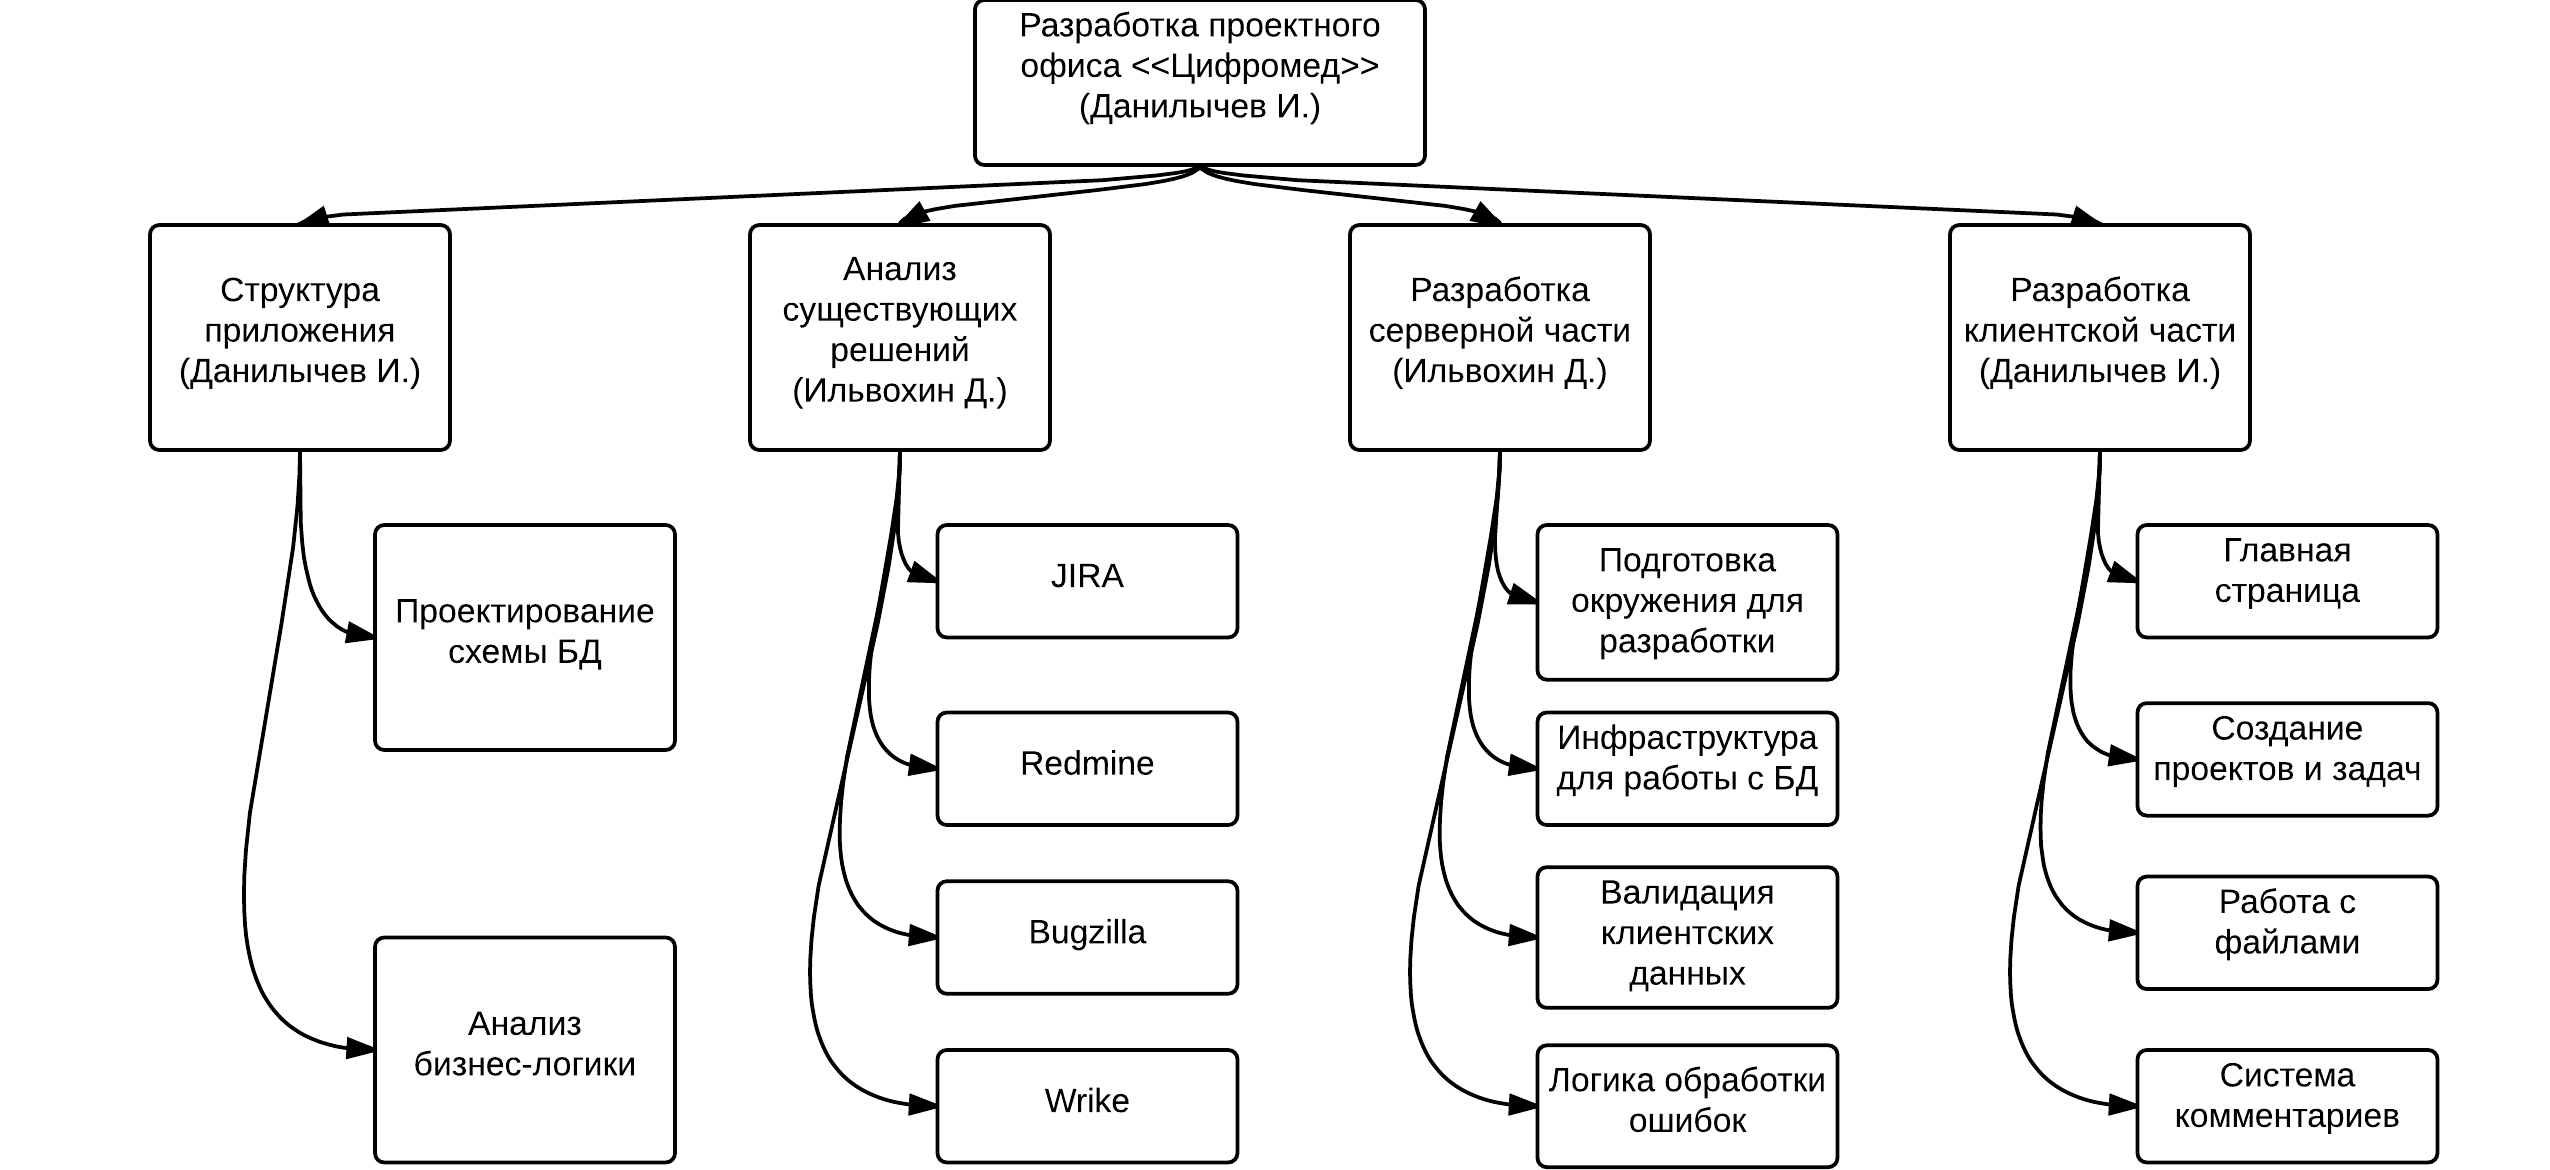
\includegraphics[scale=0.25]{../shared_images/wbs.png}
    \caption{Cтруктура декомпозиции работ проекта}
    \label{fig:wbo}
\end{figure}

\chapter{\MakeTextUppercase{Сравнение существующих решений}}
Управление проектами --- в соответствии с определением национальным стандартом
ANSI PMBoK — область деятельности, в ходе которой определяются и достигаются
четкие цели проекта при балансировании между объёмом работ, ресурсами 
(такими как деньги, труд, материалы, энергия, пространство и др.), временем, качеством и рисками. 
Ключевым фактором успеха проектного управления является наличие чёткого заранее определённого плана,
минимизации рисков и отклонений от плана, эффективного управления изменениями.~\cite{wiki_pm}

\section{\MakeTextUppercase{Задачи программного обеспечения для управления проектами}}
Для достижения конечных целей проекта менеджеру проекта необходимо специальное программное обеспечение
для управления проектом или портфелем проектов.
Задачи программного обеспечения такого рода обычно делят на три части:
\begin{itemize}
\item планирование;
\item управление данными и предоставление информации;
\item управление коммуникациями команды проекта.
\end{itemize}

\subsection{\MakeTextUppercase{Планирование}}
Одной из наиболее распространенных и на мой взгляд наиболее важных возможностей
программного обеспечения для управления проектами является возможность планирования
событий и управления задачами. Требования могут различаться в зависимости от того
для каких целей и проектов используется инструмент, наиболее распространенными являются:
\begin{itemize}
\item планирование различных событий, зависящих друг от друга;
\item идентификация крупных составных частей проекта (вехи проекта) и их декомпозиция, посредством которой создается структура декомпозиции работ, также называемая иерархической структурой работ (англ. Work Breakdown Structure, WBS)~\cite{pmbok};
\item планирование расписания работы сотрудников и назначение ресурсов на конкретные задачи;
\item расчет времени, необходимого на решение каждой из задач;
\item сортировка задач в зависимости от сроков их завершения;
\item презентация графика работ по проекту в виде диаграммы Ганта (рисунок ~\ref{fig:gantt_ex});
\item управление нескольким проектами одновременно.
\end{itemize}

\begin{figure}[!htb]
  \centering
    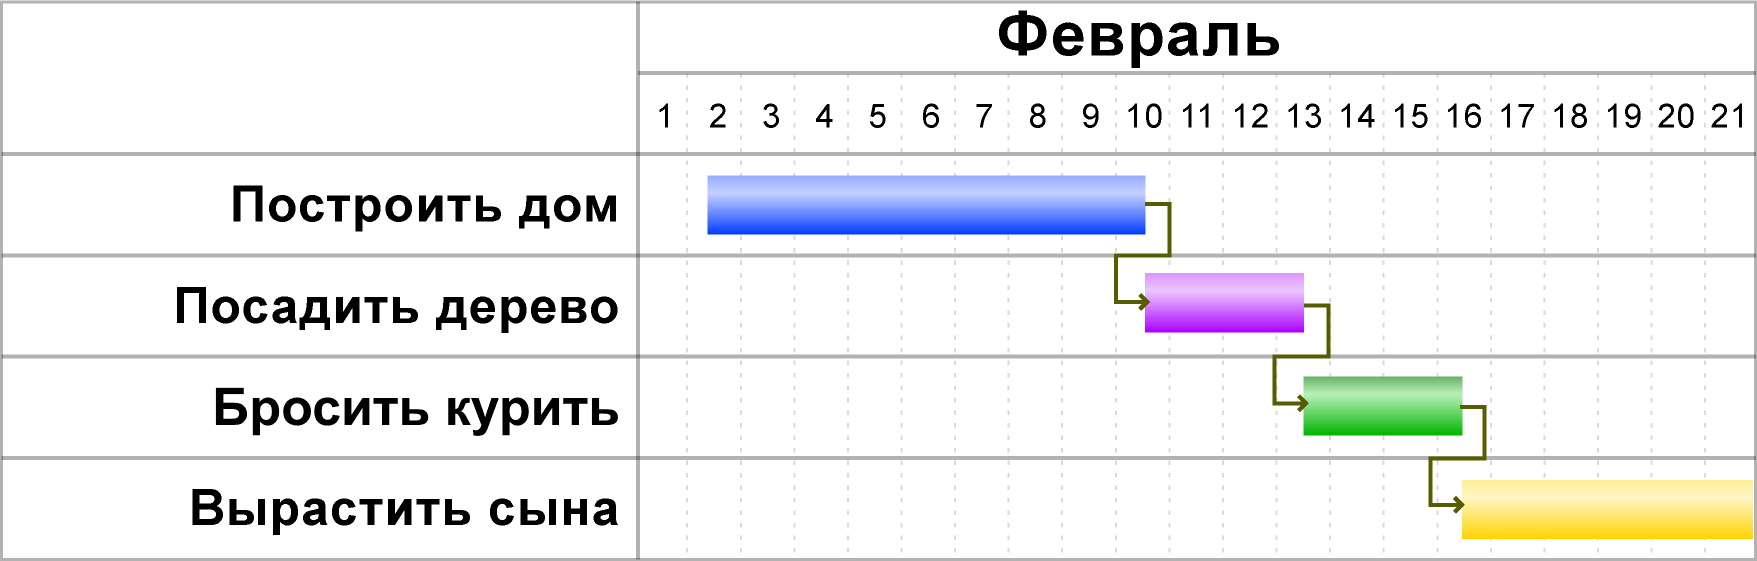
\includegraphics[scale=0.25]{pics/gantt.png}
    \caption{Пример диаграммы Ганта}
    \label{fig:gantt_ex}
\end{figure}

Для реализации в прототипе нашей системе мы выбрали несколько, по нашему мнению, самых важных возможностей
из этого списка.

\subsection{\MakeTextUppercase{Управление данными и предоставление информации}}
Программное обеспечение для управления проектами предоставляет большое количество
требуемой информации, такой как:
\begin{itemize}
  \item список задач для сотрудников и информацию распределения ресурсов;
  \item обзор информации о сроках выполнения задач;
  \item ранние предупреждения о возможных рисках, связанных с проектом;
  \item информации о рабочей нагрузке;
  \item информация о ходе проекта, показатели и их прогнозирование.
\end{itemize}

\subsection{\MakeTextUppercase{Управление коммуникациями команды проекта}}
\begin{itemize}
  \item обсуждение и согласование рабочих вопросов проекта;
  \item фиксация проблем проекта и запросов на изменения, их обработка;
  \item ведение рисков проекта и управление ими;
  \item предоставление доступа к информации о ходе проекта в виде живой ленты событий.
\end{itemize}

\section{\MakeTextUppercase{Типы программного обеспечения для управления проектами}}
\subsection{\MakeTextUppercase{Настольные}}
Программное обеспечение для управления проектами реализовано в виде настольного приложения,
которое запускается на персональном компьютере каждого пользователя. Обычно, настольное
программное обеспечение для управления проектами реализовано в виде однопользовательского
приложения, которое использует проектный менеджер или какой-то другой заинтересованный
сотрудник, например, риск-менеджер.

\subsection{\MakeTextUppercase{Веб-приложения}}
Программное обеспечение для управления проектами реализовано в виде веб-приложения,
которое доступно при помощи веб-браузера. Как правило, приложения такого рода доступны
для использования с помощью смартфона или планшета. Software as a Service (SaaS) так же
является веб-приложением, такая модель использования становится все более популярной
для бизнес-приложений, включая системы управления информацией проекта и управления
портфолио проекта. Обычно SaaS решения доступны для использования так же с помощью
веб-браузера.

\subsection{\MakeTextUppercase{Персональные}}
Персональные приложения для управления проектами используются дома, обычно, для
управления <<ежедневными>> задачами или домашними проектами. Персональные приложения
сильно пересекаются с однопользовательскими, но их основное отличие заключается в
предоставлении более простого интерфейса пользователя, нацеленного на простое
использование приложения непрофессионалами.
\subsection{\MakeTextUppercase{Однопользовательские}}
Однопользовательские системы реализованы на основе предположения, что в один момент
времени только один пользователь будет редактировать информацию проекта. Системы такого
рода могут быть использованы в маленьких компаниях или в компаниях где всего несколько
человек занимается задачами управления проектами. Как правило, настольные приложения
попадают в эту категорию.

\subsection{\MakeTextUppercase{Многопользовательские}}
Многопользовательские системы поддерживают редактирование нескольких проектных
планов или даже разных частей одного плана несколькими пользователями одновременно.
Например, обновление области личной ответственности части проектного плана, которая
будет интегрирована в общий проектный план. Веб-приложения попадают в эту категорию,
но у них есть существенное ограничение: приложения такого типа могут быть использованы
только, когда у пользователя есть подключение к сети Интернет. Для обхода этого
ограничения, некоторые приложения используют полноценное настольное приложение, которое
установлено на персональном компьютере пользователя и которое периодически подключается
к центральному серверу, для сохранения изменений, которые сделал пользователь и получения
изменений, сделанных в это время другими пользователями системы.

\subsection{\MakeTextUppercase{Сводная таблица}}
Для сравнения программного обеспечения для управления проектами было выделено
несколько пунктов:
\begin{enumerate}
\item Лицензия. Для использования приложения необходимо заплатить деньги
  его разработчикам, если это проприетарное программное обеспечение, как правило,
  при такой лицензии самостоятельная доработка продукта невозможна, потому
  что авторы приложения не распространяют его исходные коды или распространяют, но
  явно запрещают его изменение. При свободной лицензии,
  напротив, возможна самостоятельная доработка.
\item Язык реализации. У некоторых языков программирования, для больших приложений
  большой оверхед использования ресурсов, соответственно для развертывания приложения
  потребуется больше дорогих вычислительных мощностей.
\item Интерфейс. Чем больше возможностей доступа к приложению имеет пользователь --- тем лучше.
  Как правило, удобство использования приложения это первое на что обращает внимание пользователь,
  и в зависимости от своего впечатления делает выбор в пользу какого-то приложения.
\item База данных. Нам как разработчикам приложения было интересно, на основе каких баз данных
  работают существующие/популярные системы, поэтому этот пункт тоже был включен в сравнительную таблицу.
\end{enumerate}

\begin{table}[!htb]
  \caption{Сравнение систем управления проектами~\cite{jira_off}~\cite{redmine_off}~\cite{bugzilla_off}~\cite{wrike_off}}
  \label{tab:cmp_pm}
  \begin{center}
    \begin{tabularx}{\textwidth}{|l|X|X|X|X|}
      \hline
      Система & Лицензия & Язык реализации & Интерфейс & БД \\
      \hline
      JIRA & проприетарное ПО & Java & Web, e-mail, RSS & MySQL, Oracle, PostgreSQL, MS SQL Server и др. \\
      \hline
      Redmine & GPL v2 & Ruby on Rails & Web, E-mail, Atom, iPhone, Windows Phone, Android & MySQL, PostgreSQL, SQLite \\
      \hline
      Bugzilla & MPL & Perl & Web, e-mail, RSS, Web service, cli, iPhone & MySQL, PostgreSQL \\
      \hline
      Wrike & проприетарное ПО & Java & Web, email & PostgreSQL \\
      \hline
      Цифромед & свободная & Python & Web & CouchDB \\
      \hline
    \end{tabularx}
  \end{center}
\end{table}

Для полноты сравнения в таблицу~\ref{tab:cmp_pm} добавлено приложение, разработанное нами.

Ключевым столбцов в сравнении различных систем мы рассматривали поле --- интерфейс.
Понятно, что чем больше возможностей имеет пользователь для доступа к приложению, тем лучше,
но мы физически не смогли бы реализовать интерфейсы для всех возможных платформ за короткий период,
поэтому решили остановиться на самом доступном и популярном Web-интерфейсе приложения.

\chapter{\MakeTextUppercase{Подготовка окружения для разработки}}
Для совместной разработки проекта была выбрана децентрализованная система контроля
версий --- git, которая была создана Линусом Торвальдсом для управления разработкой
ядра Linux.~\cite{git_home}

Для разработки проекта было решено не поднимать git на собственном сервере, а использовать
готовую платформу Github.

При разработке системы решили использовать модель разработки, предложенную Винсентом
Дрессэнем (англ. Vincent Driessen).~\cite{git_branching_model}

Основной идеей этой модели разработки является то, что все изменения происходят в
<<develop>> ветке, от которой (когда разработка всех новых возможностей, которые
должны попасть в релиз закончена) отводится релизная ветка, изменения из которой
вносятся в <<master>> ветку, которая считается стабильной в любой момент времени.
Более подробно модель разработки разобрана на рисунке~\ref{fig:branching}.
Пока мы находимся на ранней стадии разработки до версии 0.1, поэтому вносим все изменения
в <<master>> ветку. % :D

\begin{figure}[!htb]
  \centering
    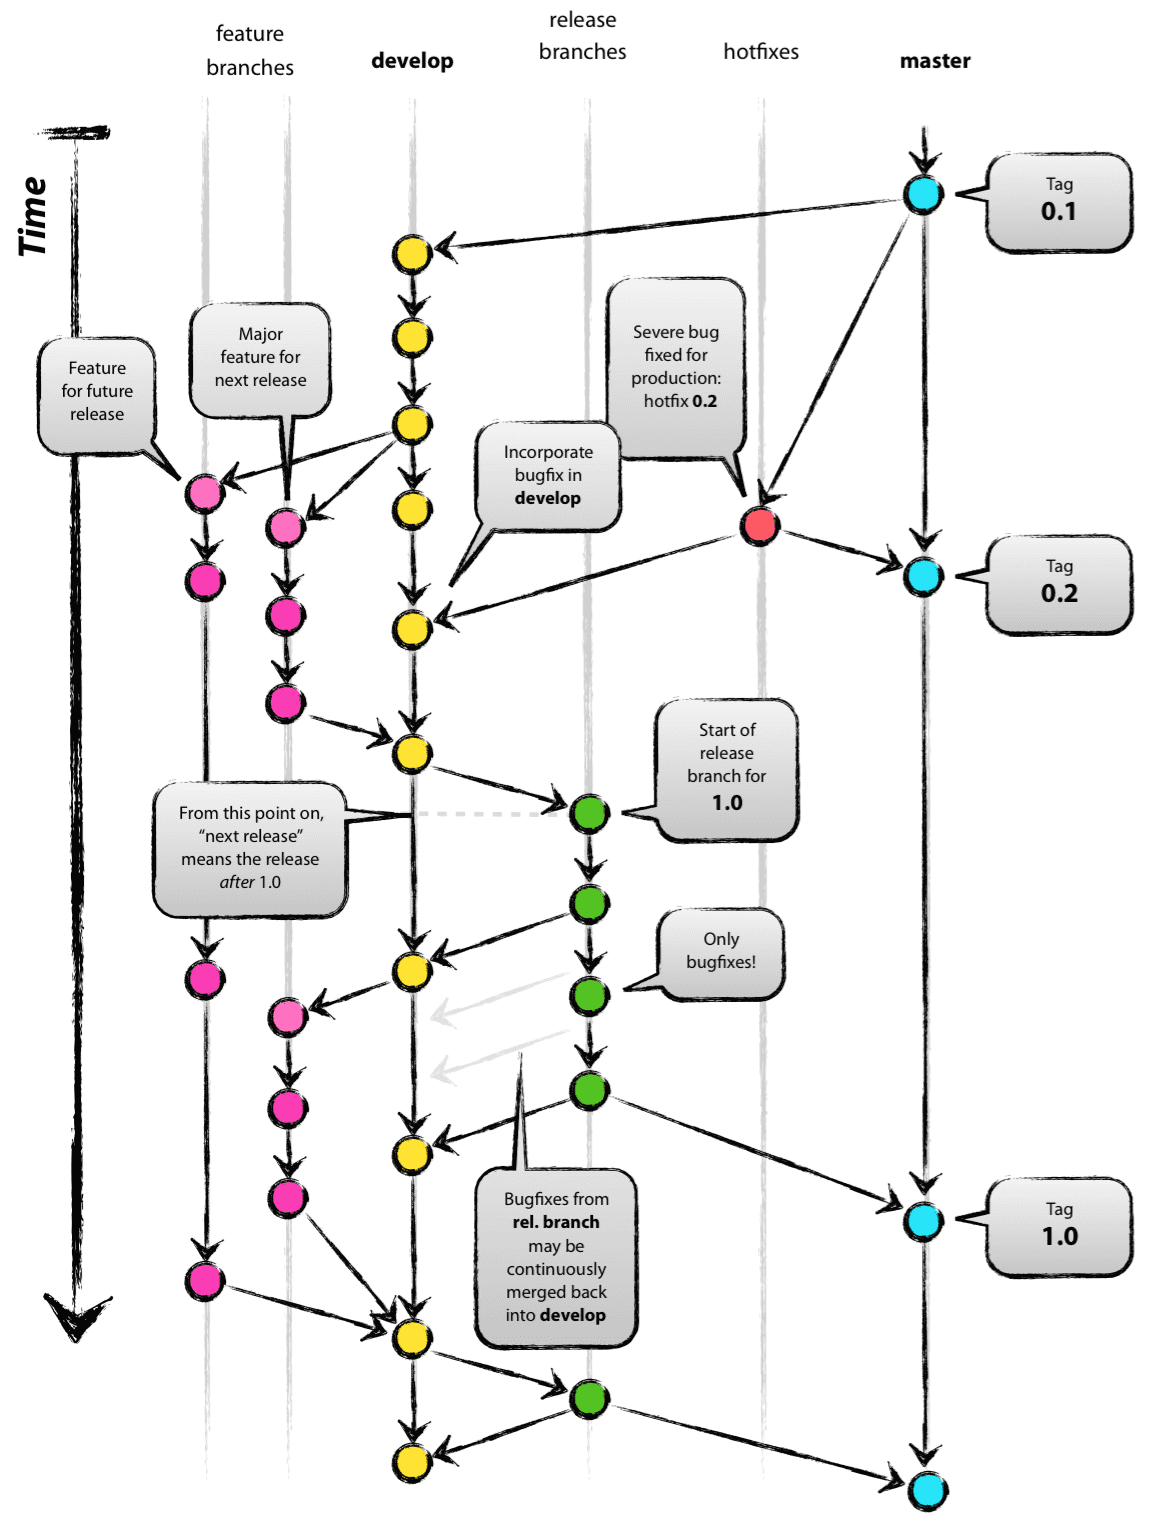
\includegraphics[scale=0.3]{pics/branching.png}
    \caption{Модель разработки}
    \label{fig:branching}
\end{figure}

\chapter{\MakeTextUppercase{Разработка серверной части}}
Несмотря на то, что большинство существующих систем использует реляционные
базы данных, в своем проекте мы решили отказаться от традиционного подхода
к базе данных и использовать, современный, набирающий в последнее время популярность
NoSQL подход. NoSQL решения для управления большими данными используют гиганты индустрии,
такие как: IBM, Facebook, Netflix, EBay, Hulu, Yahoo!, благодаря поддержке которых технология
широко распространилась за последние несколько лет.

В разработке нашего решения для управления проектами мы использовали документоориентированную
систему управления базами данных Apache CouchDB.

Документоориентированные СУБД специально предназначены для хранения иерархических структур
данных (документов). В основе документоориентированных СУБД лежат документные хранилища (англ. document store),
имеющие структуру дерева (иногда леса).

Такой подход очень подходит для построения системы управления проектами, которая тоже имеет древовидную с структуру:
корень дерева --- проект, его узлы --- задачи, пример структуры приведен на рисунке~\ref{fig:project_tree}.

\begin{figure}[!htb]
  \centering
    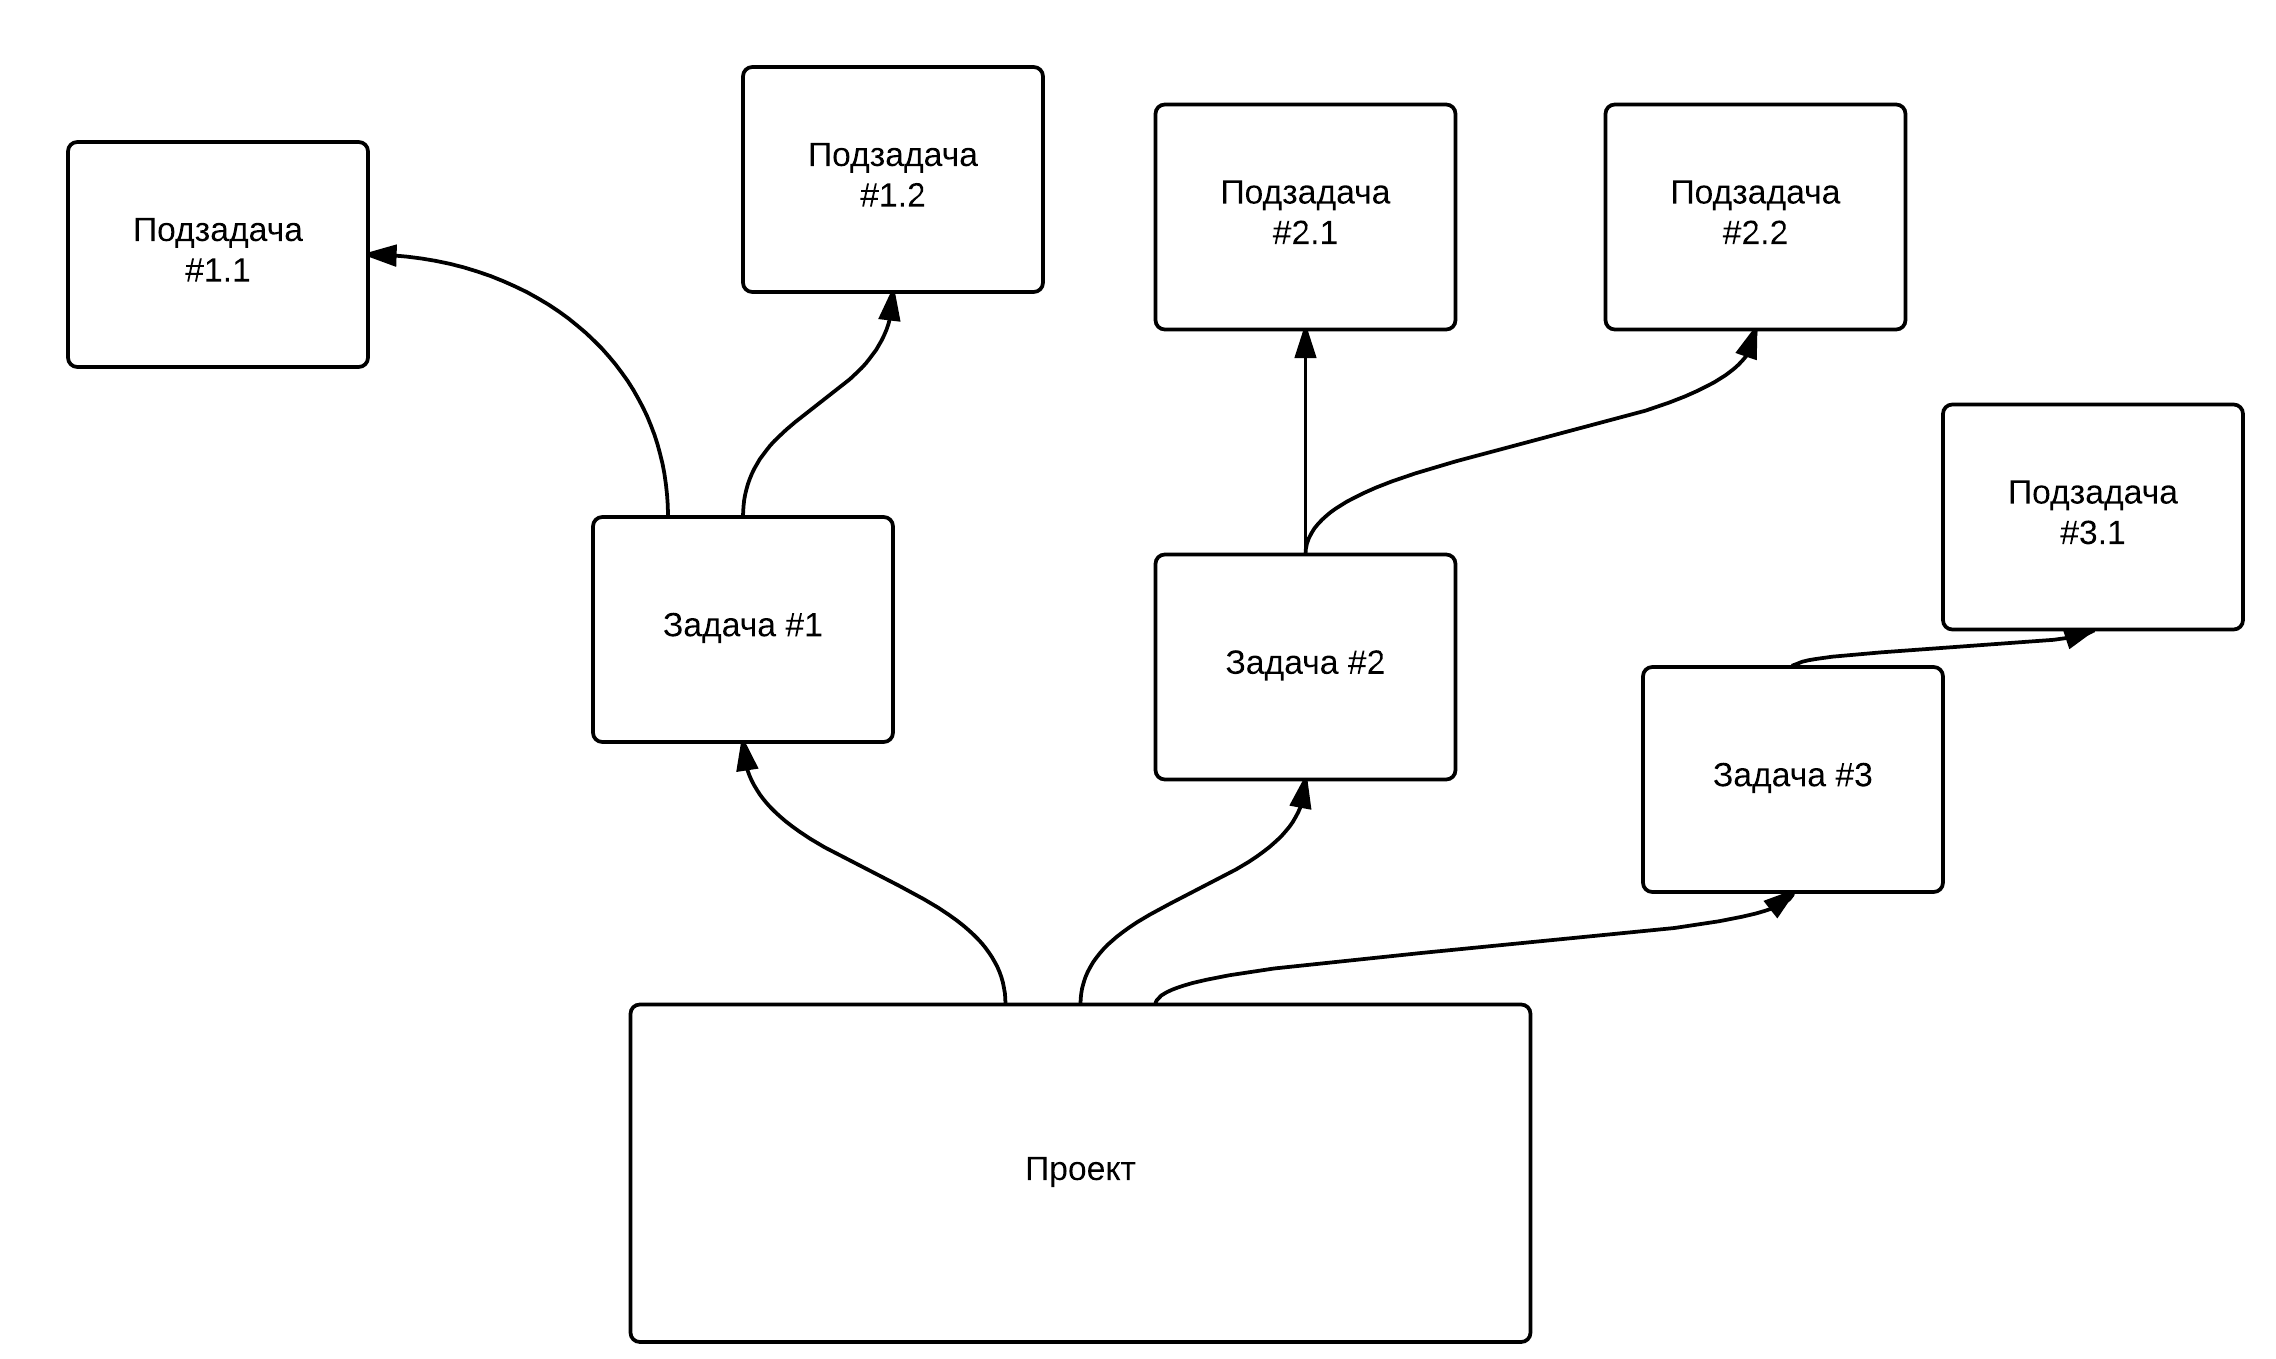
\includegraphics[scale=0.2]{../slides/images/test_tree.png}
    \caption{Структура проекта}
    \label{fig:project_tree}
\end{figure}

В отличие от реляционного подхода к созданию и управлению базами данных для которых
нужно разработать схему со множеством таблиц и сложными отношениями между ними, в
документоориентированной БД в этом нет необходимости, все данные хранятся вместе в
отдельных документах без какой-либо заранее составленной схемы, диаграмма~\ref{fig:rel_vs_doc}
иллюстрирует отличия в данных подходах.

\begin{figure}[!htb]
  \centering
    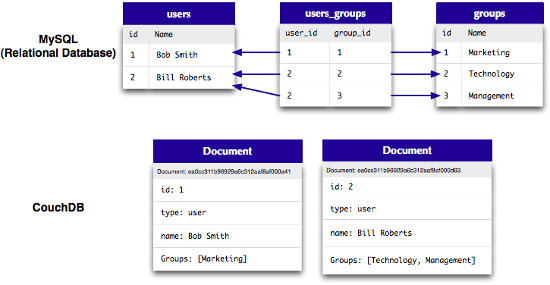
\includegraphics[scale=0.6]{pics/rel_vs_doc.png}
    \caption{Отличия хранения данных в документоориентированной и реляционной БД}
    \label{fig:rel_vs_doc}
\end{figure}

Основные особенности CouchDB:
\begin{enumerate}
\item данные хранятся не в строках и колонках, а в виде JSON-подобных документов,
  моделью которых является не таблицы, а деревья;
\item типизация элементов данных, то есть сопоставление отдельным полям документов типов INTEGER, DATE и пр.,
  не поддерживается — вместо этого пользователь может написать функцию-валидатор;
\item целостность базы данных обеспечивается исключительно на уровне отдельных записей
  (но не на уровне связей между ними);
\item для построения индексов и выполнения запросов используются функции представления (view)~\cite{couchdb_doc};
\item функции-валидаторы, функции-представления, функции-фильтры сохраняются в текстовом виде в самой базе данных.
\end{enumerate}

Для использования данных из CouchDB в коде приложения мы использовали технологию подобную ORM,
которая связывает базу данных с концепциями объектно-ориентированных языков программирования,
таким образом как бы создавая <<виртуальную объектную базу данных>>.

\chapter{\MakeTextUppercase{Заключение}}
Благодаря анализу существующих решений программного обеспечения для управления проектами,
перед началом разработки, нам удалось выделить основные и самые востребованные в настоящее
время возможности существующих продуктов и внести их в техническое задание, как обязательные
для реализации в разрабатываемом нами приложении.

В рамках задачи подготовки рабочего окружения была развернута инфраструктура и выбрана
модель разработки, которые использовались на протяжении всего процесса разработки приложения.

При разработке серверной части приложения была использована наиболее подходящая под нужды
нашего проекта система управления базами данных, благодаря чему удалось существенно сократить
время на написание кода для взаимодействия с базой данных и упростить процесс разработки.

\newpage
\clearpage
%
\addcontentsline{toc}{chapter}{\MakeTextUppercase{Список использованных источников}}
\begin{thebibliography}{}
\bibitem{wiki_pm} Википедия [Электронный ресурс]: \\https://ru.wikipedia.org/wiki/Управление\_проектами
\bibitem{pmbok} Руководство к своду знаний по управлению проектами (руководство PMBOK 4 издание), с. 204
\bibitem{jira_off} Официальный сайт системы Atlassian JIRA [Электронный ресурс]: https://www.atlassian.com/software/jira
\bibitem{redmine_off} Официальный сайт системы Redmine [Электронный ресурс]: http://www.redmine.org
\bibitem{bugzilla_off} Описание возможностей на официальном сайте системы Bugzilla [Электронный ресурс]: https://www.bugzilla.org/features
\bibitem{wrike_off} Документация на официальном сайте системы Wrike [Электронный ресурс]: https://developers.wrike.com/documentation/api/overview
\bibitem{git_home} Домашняя страница Git [Электронный ресурс]: http://git-scm.com
\bibitem{git_branching_model} Vincent Driessen, A successful Git branching model [Электронный ресурс]: http://nvie.com/posts/a-successful-git-branching-model
\bibitem{couchdb_doc} Серверы представлений: документация Apache CouchDB [Электронный ресурс]: http://wiki.apache.org/couchdb/ViewServer
\end{thebibliography}

\end{document}
